% !TEX root =  podc-submission.tex

\section{Queue Implementation} \label{DescriptQ}

We use a static {\it tournament tree}, which is a static binary tree of height $\ceil{\log_2 p}$ with one leaf 
assigned to each process. 

There is a shared binary tree among the processes to agree on one
total ordering of the operations invoked by processes. The tree is
called a \it{tournament tree} (see Figure~\ref{fig::blocktree}). Each
process has a leaf in which the operations invoked by the process are
stored in order. When a process wishes to do an operation it appends
the operation to its leaf and tries to propagate its new operation up
to the tree's root. Each node of the tree keeps an ordering of
operations propagated up to it. All processes agree on the sequence of
operations in the root and this ordering is used as the linearization
ordering. 

Each of the processes $P_1,P_2,...,P_p$ has a leaf and in each node
there is an ordering of operations stored. Each process tries to
propagate its operations up to the root, which stores a total ordering
of all operations. 

To propagate operations to a node $n$ in the tree, a process observes
the operations in both of $n$'s children that are not already in $n$,
merges them to create an ordering and then tries to append the
ordering to the sequence stored in $n$. We call this procedure
\tt{$n$.Refresh} (see Figure \ref{fig::propagstep}). A \nf{Refresh} on
$n$ with a successful append helps to propagate their operations up to
$n$. We shall prove that if a process invokes \tt{Refresh} on the node
$n$ two times and fails to append the new operations to $n$ both
times, the operations that were in $n$'s children before the first
\tt{Refresh} are guaranteed to be in $n$ after the second failed
\tt{Refresh}. 
We sketch the argument here.

\begin{figure}[hbtp]
\begin{center}
\hspace{6em}\begin{subfigure}[b]{.29\textwidth}
  \centering
  \resizebox{\columnwidth}{!}{
  \begin{tikzpicture}[level 1/.style={level distance=1.2cm,sibling distance=0.5cm}]
\Tree [.$r_1,l_1,l_2,r_2,l_3$
$l_1,l_2,l_3,l_4,l_5$
$r_1,r_2,r_3,r_4$ ]
\end{tikzpicture}}
  \caption{Before the \nf{Refresh}.}
\end{subfigure}
\hfill
\begin{subfigure}[b]{.29\textwidth}
  \centering
  \resizebox{\columnwidth}{!}{
  \begin{tikzpicture}[level 1/.style={level distance=1.2cm,sibling distance=0.5cm}]
\Tree [.$r_1,l_1,l_2,r_2,l_3,l_4,l_5,r_3,r_4$
$l_1,l_2,l_3,l_4,l_5$
$r_1,r_2,r_3,r_4$ ]
\end{tikzpicture}}
  \caption{After the \nf{Refresh}.}
\end{subfigure}
\hspace{6em}
\caption[A successful \nf{Refresh}.]{\label{fig::propagstep} Before
  and after a \nf{$n$.Refresh} with a successful append. Operations
  propagating from the left child are labelled with $l$ and from the
  right child with $r$.} 
\end{center}
\end{figure}

\begin{figure}[hbpt]
  \center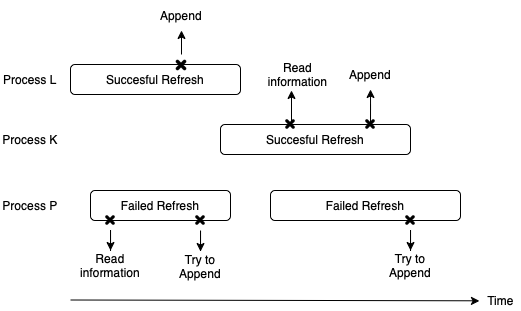
\includegraphics[width=4in]{pics/doublyrefresh-drawio.png}
  \caption[Two consecutive failed \nf{Refresh}es by a
    process.]{\label{fig::simpleDoubleRefresh}Time relations between
    the concurrent successful \nf{Refresh}es and the two consecutive
    failed \nf{Refresh}es.} 
\end{figure}

We use \nf{CAS} (Compare\&Swap) instructions to implement the
\nf{Refresh}'s attempt to append  described in the previous
paragraph. 
The second failed \nf{Refresh} of $P$ is assuredly concurrent with a
successful \texttt{Refresh} that has read its information after the
invocation of the first failed \nf{Refresh} (see Figure
\ref{fig::simpleDoubleRefresh}). This is because some process $L$ does
a successful append during $P$'s first failed attempt, and some
process $K$ performs a \nf{Refresh} that reads its information after
$L$'s append and then performs a successful append during $P$'s second
failed \nf{Refresh}. Process $K$'s \nf{Refresh} helps to append the
new operations that were in $n$'s children before $P$'s first failed
\nf{Refresh}, in case they were not already appended. After a process
appends its operation into its leaf it can call \nf{Refresh} on the
path up to the root at most two times on each node. So, with $O(\log
p)$ \nf{CAS}es an operation can ensure it appears in the
linearization. This cooperative solution allows us to overcome the CAS
Retry Problem. 


It is not efficient to explicitly store the sequence of operations in
each node because each operation would have to be copied all the way
up to the root; doing this would not be possible in poly-logarithmic
time. 
Instead we use an implicit representation of the operations propagated
together. Furthermore, we do not need to maintain an ordering on
operations propagated together in a node until they have reached the
root. It is sufficient to only keep track of sets of operations
propagated together in each \nf{Refresh} and then define the
linearization ordering only in the root (see Figure
\ref{fig::set}). Achieving a constant-sized implicit representation of
operations in a \nf{Refresh} allows us to do \texttt{CAS} instructions
on fixed-size objects in each \tt{Refresh}. To do that, we introduce
\it{block}s. A block stores information about the operations
propagated by a \nf{Refresh}. It contains the number of operations
from the left and the right child propagated to the node by the
\texttt{Refresh} procedure. See Figure~\ref{fig:block} for an
example. A node stores an array of blocks of operations propagated up
to it. A propagate step  aggregates the new blocks in the children
into a new block and stores the new block in the parent. We call the
aggregated blocks \it{subblocks} of the new block and the new block
the \it{superblock} of them.  In each \nf{Refresh} there is at most
one operation from each process trying to be propagated, because one
process cannot invoke two operations concurrently. Thus, there are at
most $p$ operations in a block. Furthermore, since the operations in a
\texttt{Refresh} step are concurrent we can linearize them  among
themselves in any order we wish, because if two operations are read in
one successful \tt{Refresh} step in a node they are going to be
propagated up to the root together. Our choice is to put the
operations propagated from the left child before the operations
propagated from the right child. In this way, if we know the number of
operations from the left child and the number of operations from the
right child in a block, we have a complete ordering of the
operations. 

\begin{figure}[hbtp]
\begin{center}
\begin{tikzpicture} [level 1/.style={level distance=1.8cm,sibling distance=0.6cm}, level 2/.style={level distance=1.4cm,sibling distance=0.4cm}]
  
\Tree [.{$\big\{op_2^1,op_1^1,op_3^1\big\},\big\{op_4^1$, $op_3^2\big\},\big\{op_2^2, op_4^2\big\},\big\{op_1^2\big\}...$ }  [.{ $\big\{op_2^1, op_1^1\big\},\big\{op_2^2\big\},\big\{op_1^2\big\}...$ }
      {\begin{tabular}{|l|c|c|c}  \hline $op_1^1$ & $op_1^2$ & ... \\ \hline\end{tabular}} {\begin{tabular}{|l|c|c|c}  \hline $op_2^1$ & $op_2^2$ & ... \\ \hline \end{tabular}} ] [.{ $\big\{op_3^1\big\},\big\{op_4^1$, $op_3^2\big\},\big\{op_4^2\big\},...$ } {\begin{tabular}{|l|c|c|c}  \hline $op_3^1$ & $op_3^2$ & ... \\ \hline\end{tabular}} {\begin{tabular}{|l|c|c|c} \hline $op_4^1$ & $op_4^2$ & ... \\ \hline\end{tabular}} ] ]
\end{tikzpicture}
\caption[The operations merged in a \nf{Refresh} step with
  sets.]{\label{fig::set} Leaves are for processes $P_1$ to $P_4$ from
  left to right. In each internal node one can arbitrarily linearize
  the sets of concurrent operations  propagated together in a
  \nf{Refresh}. For example $op_4^1$ and $op_3^2$ have propagated
  together in one \nf{Propagate} step and they will be propagated up
  to the root together. Since their execution time intervals overlap,
  they can be linearized in any order.} 
\end{center}
\end{figure}


\begin{figure}[hbtp]
\begin{center}
\begin{tikzpicture}
[level 1/.style={level distance=3.3cm,sibling distance=0cm},
	level 2/.style={level distance=2.5cm,sibling distance=0cm},
	level 3/.style={level distance=1.7cm,sibling distance=2cm}]
\begin{small} 

\Tree [.{\begin{tabular}{|c|c|c|}  \hline (0,11) & (12,6) & (8,36) \\ \hline\end{tabular}}
 [.{\begin{tabular}{||c||c||}  \hline (10,2) & (5,3) \\\hline  \end{tabular}}
 [.{\begin{tabular}{||c|c||c||}\hline (2,3) & (4,1) & (0,5) \\\hline\end{tabular}} $\vdots$ $\vdots$ ]
  [.{\begin{tabular}{||c||c||}  \hline (0,2) & (1,2)  \\ \hline  \end{tabular}} $\vdots$ $\vdots$ ] ]
          [.{\begin{tabular}{||c||c||c|c||}  \hline (3,8) & (6,0) & (14,6) & (0,16) \\ \hline \end{tabular}}
           [.{\begin{tabular}{||c||c||c|c||}  \hline (0,3) & (4,2) & (5,1) & (3,5) \\ \hline \end{tabular}} $\vdots$ $\vdots$ ]
            [.{\begin{tabular}{||c|c||c||c||}  \hline (2,1) & (5,0) & (4,2) & (9,7) \\ \hline \end{tabular}} $\vdots$ $\vdots$ ] ] ]
\end{small}
\end{tikzpicture}
\end{center}
\caption[The operations merged in a \nf{Refresh} step with (left,
  right) blocks.]{\label{fig:block} Using blocks to represent
  operations. Blocks between two lines $||$ are propagated together to
  the parent. Each block consists of a pair (left, right) indicating
  the number of operations from the left and the right child,
  respectively. For example, (12,6) in the root contains  (10,2) from
  the left child and (6,0) from the right child. The third block in
  the root (8,36) is created by merging (5,3) from the left child and
  (14,6) and (0,16) from the right child. (5,3) is the superblock of
  (0,5) and (1,2) and (5,1),(3,5) and (4,2) are subblocks of (14,6).} 
\end{figure}

So far, we have a shared tree that processes use to agree on the
implicit ordering stored in its root. With this agreement on the
linearization ordering, we can design a universal construction; for a
given object, we can perform an operation $op$ by applying all the
operations up until $op$ in the root on a local copy of the object and
then returning the response for $op$. However, this approach is not
enough for an efficient queue. 
We show that we can build an efficient queue if we can compute two
things about the ordering in the root: (1) the $i$th propagated
operation and (2) the rank of a propagated operation in the
linearization. We explain how to implement (1) and (2) in
poly-logarithmic steps. 

After propagating an operation \textit{op} to the root, processes can
find out information about the linearization ordering using (1) and
(2).  
To get the $i$th operation in the root, we find the block $B$
containing the $i$th operation in the root, and then recursively find
the subblock of $B$ in the descendent of the root that contains that
$i$th operation. When we reach a block in a leaf, the operation is
explicitly stored there. To make this search faster, instead of
iterating over all blocks in the node, we store the prefix sum of the
number of elements in the blocks sequence to permit a binary search
for the required block. We also store pointers to determine the range
of subblocks of a block to make the binary search faster. In each
block, we store the prefix sum of operations from the left child and
from the right child. Moreover, for each block, we store two
attributes \nf{end\sub{left}} and \nf{end\sub{right}}, the indices of
the last left and right subblock (see Figure \ref{fig::pointer}). We
know a block size is at most $p$, so binary search takes at most
\textsc{O}$(\log p)$ time, since the \nf{end\sub{left}} and
\nf{end\sub{right}} indices of a block and its previous block reduce
the search range size to \textsc{O}$(p)$. 

To compute the rank in the root of an operation in a leaf, we need to
find the superblock of the block that the operation is in. After a
block is installed in a node we store the approximate index of its
superblock in it to make this faster. 

\begin{figure}[hbtp]
\centering
  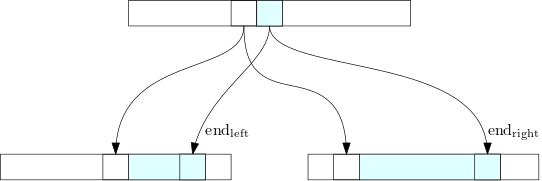
\includegraphics[width=4in, height=1.4in]{pics/pointers}
  \caption{Each block stores the index of its last subblock in each
    child. \label{fig::pointer}} 
\end{figure}

In an execution on a queue where no dequeue operation returns
\nf{null}, the $k$th dequeue returns the argument of the $k$th
enqueue. In the general case a dequeue returns \nf{null} if and only
if the queue size after the previous operation is 0. We refer to such
a dequeue as a \it{null dequeue}. If the dequeue is the $k$th non-null
dequeue, it returns the argument of the $k$th enqueue. Having the size
of the queue after an operation we can compute the number of non-null
dequeues from the number of enqueues before the operation. So, if we
store the size of the queue after each block of operations in the
root, we can compute the index of the enqueue whose argument is the
response to a given dequeue in constant time. 

In our case of implementing a queue, a process only needs to compute
the rank of a \nf{Dequeue} and get an \nf{Enqueue} with a specific
position.  We know we can linearize operations in a block in any
order; here, we choose to put \nf{Enqueue} operations in a block
before \nf{Dequeue} operations. Consider the following operations,
where operations in a cell are concurrent. 
\begin{table}[hbtp]
\centering
\begin{small}
\begin{tabular}{c|c|c|c}
    \hline \texttt{Deq} & \texttt{Enq(5)}, \texttt{Enq(2)}, \texttt{Enq(1)}, \texttt{Deq}& \texttt{Enq(3)}, \texttt{Deq}&  \texttt{Enq(4)}, \texttt{Deq}, \texttt{Deq}, \texttt{Deq}, \texttt{Deq}\\ \hline
  \end{tabular}
\end{small}
\caption{An execution on a queue separated by the operations in the root blocks.}
\end{table}

\noindent The \texttt{Dequeue} operations return \texttt{null, 5, 2,
  1, 3, 4, null}, respectively. 
Now, we claim that by knowing the size of the queue, we can compute
the rank of the required \texttt{Enqueue} for any non-null
\nf{Dequeue}. We apply this approach to blocks; if we store the size
of the queue after each block of operations, we can compute the index
of each \nf{Dequeue}'s result in \textsc{O}$(1)$ steps. 

\begin{table}[hbtp]
\centering
\begin{small}
  \begin{tabular}{c|c|c|c|c}
    \hline &\texttt{Deq} & \texttt{Enq(5)}, \texttt{Enq(2)}, \texttt{Enq(1)}, \texttt{Deq}& \texttt{Enq(3)}, \texttt{Deq}&  \texttt{Enq(4)}, \texttt{Deq}, \texttt{Deq}, \texttt{Deq}, \texttt{Deq}\\ \hline
    \#\tt{Enq}s & 0 & 3 & 1 & 1 \\ \hline
    \#\tt{Deq}s & 1 & 1 & 1 & 4 \\ \hline
    Size at end & 0 & 2 & 2 & 0 \\ \hline
  \end{tabular}
\end{small}
  \caption{Augmented history of operation blocks on the queue.}
\end{table}

\noindent The size of the queue after the $b$th block in the root
could be computed as 
$$\textrm{max}\Big(\textrm{size after }(b-1)\textrm{th block} +
\#\textrm{\tt{Enqueue}s in }b\textrm{th block} -
\#\textrm{\tt{Dequeue}s in }b\textrm{th block}, 0\Big).$$ 
\noindent Moreover, the total number of non-null dequeues in blocks
$1,2,...,b$ in the root is 
$$ \sum_{i=1}^{b} \#\textrm{\tt{Enqueue}s in }i\textrm{th block} -
\textrm{size after }b\textrm{th block}.$$ 

Given a \texttt{Dequeue} is in block $B$, its response is the argument
of the \tt{Enqueue} whose rank is 
\begin{center}
    \#\textrm{non-null } \nf{Dequeue}s in  blocks $1,2,...,b-1 +  $index of the \nf{Dequeue} among B\textrm{'s} \nf{Dequeue}
\end{center}
if \vspace{-3em}
\begin{center}
    $\big ($size of the queue after $b-1\textrm{th block} + \#\textrm{\tt{Enqueue}s in }b\textrm{th block} $\\$- \textrm{index of \tt{Dequeue} in }B\textrm{'s \tt{Dequeue}s} \big )\geq 0$.
\end{center}
Otherwise, the response would be \nf{null}.


\subsection{Details of the Implementation}
Section \ref{algQ} gives the pseudocode for the queue
implementation. It uses the following two types of objects. 
\paragraph{\tt{Node}} 
 In each \texttt{Node} we store pointers to its parent and its left
 and right child, an array of \nf{Block}s called \texttt{block}s and
 the index \nf{head} of the first empty entry in \texttt{blocks}. 

\paragraph{\tt{Block}}
 The information stored in a \nf{Block} depends on whether  the
 \nf{Block} is in an internal node or a leaf. If it is in a leaf, we
 use a \nf{LeafBlock} which stores one operation. If a block $B$ is in
 an internal node $n$, then it contains subblocks in the left and
 right children of $n$. The left subblocks of $B$ are some consecutive
 blocks in the left child of $n$ starting from where the left
 subblocks of the block prior to $B$ ended. The right subblocks of $B$
 are defined similarly. In each \texttt{block} we store four essential
 fields that implicitly summarize which operations are in the block
 \texttt{sum\textsubscript{enq-left}},
 \texttt{sum\textsubscript{deq-left}},
 \texttt{sum\textsubscript{enq-right}},
 \texttt{sum\textsubscript{deq-right}}. The
 \texttt{sum\textsubscript{enq-left}} field is the total number of
 \nf{Enqueue} operations in the blocks before the last subblock of $B$
 in the left child. The other fields' semantics are similar. The
 \nf{end\sub{left}} and \nf{end\sub{right}} field store the index of
 the last subblock of a block in the left and the right child,
 respectively. The approximate index of the superblock of non-root
 blocks is stored in their \nf{super} field. The \texttt{size} field
 in a block in the root node stores the size of the queue after the
 operations in the block have been performed.  

We now describe the routines used in the implementation.

\paragraph{\tt{Enqueue($e$)}}
An \nf{Enqueue} operation does not return a response, so it is
sufficient to propagate the \nf{Enqueue} operation to the root and
then use its position in the linearization for future \nf{Dequeue}
operations. \nf{Enqueue($e$)} creates a \nf{LeafBlock} with
$\nf{element}=e$, sets its \nf{sum\sub{enq}} and \nf{sum\sub{deq}}
fields and then appends it to the tree. 

\paragraph{\tt{Dequeue()}}
\nf{Dequeue} creates a \nf{LeafBlock}, sets its \nf{sum\sub{enq}} and
\nf{sum\sub{deq}} fields and appends it to the tree. Then, it computes
the position of the appended \nf{Dequeue} operation in the root using
\nf{IndexDequeue} and after that finds the response of the
\nf{Dequeue} by calling \nf{FindResponse}. 

\paragraph{\tt{Append($B$)}}
The \nf{head} field is the index of the first empty slot in
\nf{blocks} in a \nf{LeafBlock}. There are no multiple write accesses
on \nf{head} and \nf{blocks} in a leaf because only the process that
the leaf belongs to appends to it. \nf{Append($B$)} adds $B$ to the
end of the \nf{blocks} field in the leaf, increments \nf{head} and
then calls \nf{Propagate} on the leaf's \nf{parent}. When
\nf{Propagate} terminates, it is guaranteed that the appended block is
a subblock of a block in the \nf{root}.  

\paragraph{\tt{Propagate()}}
\nf{Propagate} on node $n$ uses the double refresh idea described
earlier and invokes two \nf{Refresh}es on $n$ in Lines
\ref{firstRefresh} and \ref{secondRefresh}. Then, it invokes
\nf{Propagate} on \nf{$n$.parent} recursively until it reaches the
root.  

\paragraph{\tt{Refresh()} and \tt{Advance()}}
The goal of a \nf{Refresh} on node $n$ is to create a block of $n$'s
children's new blocks and append it to $n$\nf{.blocks}. The variable
\nf{h} is read from $n$\nf{.head} at Line \ref{readHead}. The new
block created by \nf{Refresh} will be inserted into
$n\nf{.blocks[h]}$. Lines \ref{startHelpChild1}--\ref{endHelpChild1}
of \nf{$n$.Refresh} help to \nf{Advance} $n$'s children. \nf{Advance}
increments the children's \nf{head} if necessary and sets the
\nf{super} field of their most recently appended blocks. The reason
behind this helping is explained later when we discuss
\nf{IndexDequeue}. After helping to \nf{Advance} the children, a new
block called \nf{new} is created in Line
\ref{invokeCreateBlock}. Then, if \nf{new} is empty, \nf{Refresh}
returns \nf{true} because there are no new operations to propagate,
and it is unnecessary to add an empty block to the tree. Later we will
use the fact that all blocks contain at least one operation. Line
\ref{cas} tries to install \nf{new}. If it was successful, all is
good. If not, it means someone else has already put a block in
$n$\nf{.blocks[h]}. In this case, \nf{Refresh} helps advance
$n$\nf{.head} to \nf{h+1} and update the \nf{super} field of
$n$\nf{.blocks[h]} at Line \ref{advance}. 


\paragraph{\tt{CreateBlock()}} \texttt{$n$.CreateBlock($h$)} is used
by \nf{Refresh} to construct a block containing new operations of
$n$'s children. 
The block \nf{new} is created in Line \ref{initNewBlock} and its
fields are filled similarly for both left and right directions. The
variable  \nf{index\sub{prev}} is the index of the block preceding the
first subblock in the child in direction \nf{dir} that is aggregated
into \nf{new}. Field \texttt{new.end\textsubscript{dir}} stores the
index of the rightmost subblock of \nf{new} in the child. Then
\nf{sum\sub{enq-dir}} is computed from the sum of the number of
\nf{Enqueue} operations in the \nf{new} block from direction \nf{dir}
and the value stored in \texttt{$n$.blocks[h-1].sum\sub{enq-dir}}. The
field \nf{sum\sub{deq-dir}} is computed similarly. Then, if \nf{new}
is going to be installed in the \nf{root}, the \nf{size} field is also
computed. 

\paragraph{\tt{IndexDequeue($b,i$)}}

A call to $n$\nf{.IndexDequeue($b,i$)} computes the block and the rank
within the block in the root of the $i$th \nf{Dequeue} of the $b$th
block of $n$. Let $R_n$ be the successful  \nf{Refresh} on node $n$
that did a successful \nf{CAS(null, $B$)} into \nf{n.blocks[$b$]}. Let
$par$ be $n$\nf{.parent}. Without loss of generality, assume for the
rest of this section that ${n}$ is the left child of $par$. Let
$R_{par}$ be the first successful \nf{$par$.Refresh} that reads some
value greater than ${b}$ for \nf{left.head} and therefore contains
${B}$ as a subblock of its created block in Line
\ref{invokeCreateBlock}. Let $j$ be the index of the block that
$R_{par}$ puts in $par$\nf{.blocks}. 
 
Since the index of the superblock of ${B}$ is not known until $B$ is
propagated, $R_n$ cannot set the \nf{super} field of ${B}$ while
creating $B$. One approach for $R_{par}$ is to set the \nf{super}
field of ${B}$ after propagating $B$ to $par$. This solution would not
be efficient because there might be up to $p$ subblocks that $R_{par}$
propagated, which need to update their \nf{super} field. However,
intuitively, once $B$ is installed, its superblock is going to be
close to \nf{$n$.parent.head} at the time of installation. If we know
the approximate position of the superblock of $B$ then we can search
for the real superblock when it is needed. Thus, \nf{$B$.super} does
not have to be the exact location of  the superblock of $B$, but we
want it to be close to $j$. We can set \nf{$B$.super} to
\nf{$par$.head} while creating $B$, but the problem is that there
might be many \nf{Refresh}es on $par$ that could happen after $R_n$
reads $par$\nf{.head} and before propagating $B$ to $par$. If $R_n$
sets \nf{$B$.super} to \nf{$par$.head} after appending $B$ to
\nf{$n$.blocks} (Line \ref{setSuper1}), $R_n$ might go to sleep at
some time after installing $B$ and before setting \nf{$B$.super}. In
this case, the next \nf{Refresh}es on $n$ and $par$ help fill in the
value of \nf{$B$.super}. 

Block $B$ is appended to \nf{$n$.blocks[$b$]} on Line \ref{cas}. After
appending $B$, \nf{$B$.super} is set on Line \ref{setSuper1} of a call
to \nf{Advance} from \nf{$n$.Refresh} by the same or another process
or by Line \ref{helpAdvance} of a \nf{$n$.parent.Refresh}. We shall
show that this is sufficient to ensure that \nf{$B$.super} differs
from the index of $B$'s superblock by at most~1. 

\paragraph{\tt{FindResponse($b, i$)}}
To compute the response of the $i$th \nf{Dequeue} in the $b$th block
of the root Line \ref{checkEmpty} computes whether the queue is empty
or not. If there are more \nf{Dequeue}s than \nf{Enqueue}s the queue
would become empty before the requested \nf{Dequeue}. If the queue is
not empty, Line \ref{computeE} computes the rank $e$ of the
\nf{Enqueue} whose argument is the response to the
\nf{Dequeue}. Knowing the response is the $e$th \nf{Enqueue} in the
root (which is before the $b$th block), we find the block and position
containing the \nf{Enqueue} operation using \nf{DoublingSearch} and
after that \nf{GetEnqueue} finds its \nf{element}. 

\paragraph{\tt{GetEnqueue($b,i$)} and \tt{DoublingSearch($e, end$)}}
We can describe an operation in a node in two ways: the rank of the
operation among all the operations in the node or the index of the
block containing the operation in the node and the rank of the
operation within that block. If we know the block and rank within the
block of an operation, we can find the subblock containing the
operation and the operation's rank within that subblock in poly-log
time. To find the response of a \nf{Dequeue}, we know about the  rank
of the response \nf{Enqueue} in the root (\nf{e} in Line
\ref{computeE}). 
We also know the \nf{e}th \nf{Enqueue} is in
\nf{root.blocks[1..end]}. \nf{DoublingSearch} uses doubling to find
the range that contains the answer block (Lines
\ref{dsearchStart}--\ref{dsearchEnd}) and then tries to find the
required indices with a binary search (Line
\ref{dsearchBinarySearch}). 
A call to \nf{$n$.GetEnqueue($b,i$)} returns the \nf{element} of the
$i$th enqueue in the $b$th block of $n$. The range of subblocks of a
block is determined using the \nf{end\sub{left}} and
\nf{end\sub{right}} fields of the block and its previous block. Then,
the subblock is found using binary search on the \nf{sum\sub{enq}}
field (Lines \ref{leftChildGet} and \ref{rightChildGet}). 

